\subsection{Training and Training Set}
\label{section:training}

The classification methods developed in this thesis are based on supervised learning. Thus, a representative training set for the used drum kit is required. This training set is developed in consideration of the analysis of the frequency spectra of different stroke types in the preceding section and the usability of the future training system integrated in Easydrum.

The training system shall be included in the existing drum configurator for e-drum sets described in section \ref{section:Easydrum}. Here, the user has to stroke each drum once, whereby he can quickly configure its drum set. Because of the incoming MIDI signal produced by the e-drum set, the once trained components can be clearly differentiated. But for an analog drum set, different strokes on the same drum or cymbal can vary, as figured out in the preceding analysis of the spectral shapes. Thus, to provide a more representative training set, different stroke types of each of the drum set's components are used for the method developed in this thesis. Nevertheless, the training of several strokes of the same stroke type shall be avoided to reduce the number of training instances to a minimum. This way, the usability for the further system is ensured.

Usually, a training set contains a lot of training instances for each possible label to handle the variance that can appear in single instances. Particularly, by the use of the FFT variances can appear because of the possible loss of information or the leakage phenomenon, which is described in section \ref{section:shortTime}. Moreover, the strokes on some of the drums and especially the cymbals can produce unstable frequency peaks, which vary between different strokes. To handle these problems, by using only one training instance per stroke type, a method has been developed. This method pre-processes a recorded drum stroke for the use as a training instance, as follows:

\begin{enumerate}
  \item The onset detection algorithm (section \ref{section:onsetdetectionmethod}) is applied to the recorded audio data $y$ to find the onsets $o$ in the recorded sound. The first found onset $o(1)$ is used for the following steps.
  \item 24 frames $y_n$ with a window size of 2048 samples are extracted from the audio data. The first frame begins on the onset $o(1)$. The following frames are each shifted by 128 samples. Thus, the last frame ends 5120 samples behind the onset $o(1)$.
  %\item Each of the extracted frames $y_n$ is Fourier transformed with a Hamming window into its frequency spectrum $F(y_n)$ by using MatLab\textsuperscript{\textregistered}s build in FFT function.
\end{enumerate}

Each of the resulting frames $y_n$ is used as a training instance. This way, it is possible to reduce the user input and the errors that appear by Fourier transforming a finite sequence.

The used window size of 2048 samples is chosen in consideration of the further classification algorithm being able to run in real-time. It needs to be equal to the window size of the further classification algorithm because the resolution of the Fourier transformed spectrum needs to be equal to gain comparable data. Also the used lock time of the onset detection algorithm needs to be considered. The lock time is set to 4096 samples. Thus, the window size for classification may not be larger than 4096 samples, because otherwise more than two onsets can appear within one frame. Contrarily, if the window size is too small, the resolution of the resulting frequency spectrum doesn't show enough details to distinguish between drums or cymbal with similar frequency properties. Also, errors can appear in the frequency spectrum if the wave  length of the analyzed stroke is greater than the extracted frame. Moreover, the size of the entire processed range of samples, which is 5120, needs special consideration. It is a result of the number of 24 generated training instances by recording and the size of the window shift of 128. The more significant and varying training instances are created, the better the results of the classification algorithm are. Thereby, the size of the transient of the shortest trained stroke is considered. Using samples located after the transient needs to be avoided because these samples would contain noise, and thus would falsify the training data.

To record the test instances for this thesis, a MatLab\textsuperscript{\textregistered} interface is built. The interface is shown in figure \ref{fig:recorderInterface}. The input is recorded with a sampling rate of 44.1 kHz and a resolution of 16 bit. 

\begin{figure}[htb]
	\centering
	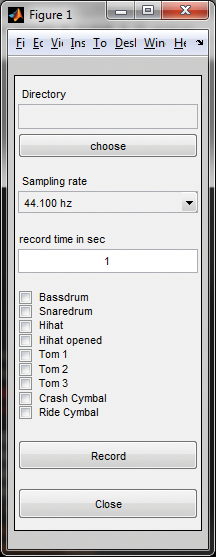
\includegraphics[width=3.6cm]{images/recorderinterface.png}
	\label{}
	\caption{Interface for recording drum sounds in MatLab\textsuperscript{\textregistered}.}
	\label{fig:recorderInterface}
\end{figure}
A training set including 696 instances is created, whereas only 29 strokes are recorded. Thereby, every stroke type of each drum and cymbal is recorded once. The drums, except for the bass drum, are trained with low powered and high powered strokes on the center and medium powered strokes at the edge of the drum head. The bass drum is only trained with a low and a high powered stroke because it can only be stroked centered. The cymbals are trained with low and high powered strokes on their rim and medium powered strokes on their bow. Moreover, low and high powered strokes on the bell of the ride drum are used as training instances. As the current Easydrum application does not distinguish between different stroke types, every drum and cymbal only has assigned a single label. Thus, the algorithm developed in this thesis only needs to be able to distinguish between the different components of the drum kit. It doesn't need to be able to differentiate varying stroke types for the same drum or cymbal. The second classification method, which is described in section \ref{section:method2}, additionally tries to differentiate between the trained stroke types.

\subsection{Test Set}
\label{section:testset}

To test the different classification methods, which are described in the following sections, a test set is created. For the test set there are recorded ten strokes for every stroke type of each drum and cymbal. This makes a total number of 290 test recordings.
